\documentclass[11pt]{article}
\usepackage[utf8]{inputenc}
\usepackage{amsmath,amssymb,amsfonts}
\usepackage{xcolor}
\usepackage{tikz}
\usepackage{amsmath}

\begin{document}

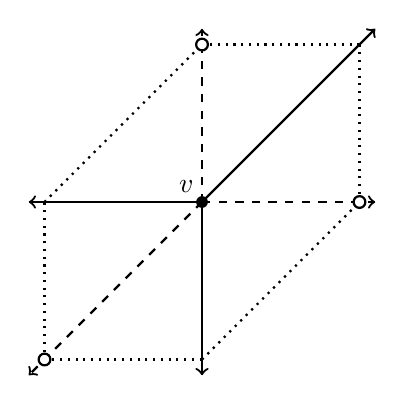
\begin{tikzpicture}[node distance={30mm}, thick, main/.style = {draw, circle}]
\draw [-,dotted](1,1) to (1,3);
\draw [-,dotted](1,1) to (3,1);
\draw [-,dotted](1,3) to (3,5);
\draw [-,dotted](3,1) to (5,3);
\draw [-,dotted](5,5) to (3,5);
\draw [-,dotted](5,5) to (5,3);
\draw [->](3,3) to (.8,3);
\draw [->](3,3) to (3,.8);
\draw [dashed,->](3,3) to (3,5.2);
\draw [dashed,->](3,3) to (5.2,3);
\draw [<-](5.2,5.2) to (3,3);
\draw [dashed,->](3,3) to (.8,.8);
\node at (1,1) [circle,draw=black,fill=white,inner sep=1.5pt]{};
\node at (5,3)[circle,draw=black,fill=white,inner sep=1.5pt]{};
\node at (3,5)[circle,draw=black,fill=white,inner sep=1.5pt]{};
\node at (3,3)[circle,fill,inner sep=1.5pt]{};
\node[] at (2.8, 3.2) {$v$};
\end{tikzpicture}

\end{document}